%% Graphical Abstract for Computers & Graphics submission
%% Design: left = method core (TCAS schedule, simplified from the paper's method figure),
%%         right = key results of the revised paper (276-object holdout framing).
%% Fonts sized so the abstract stays readable at the required 5 x 13 cm display size.
%% Compile: pdflatex graphical_abstract_CAG.tex
\documentclass[border=2pt]{standalone}
\usepackage{txfonts}
\usepackage{array}
\usepackage{tikz}
\usepackage{pgfplots}
\pgfplotsset{compat=1.16}
\usetikzlibrary{arrows.meta,positioning}

\definecolor{cagblue}{RGB}{0,82,155}
\definecolor{cagred}{RGB}{196,30,30}
\definecolor{caggreen}{RGB}{20,120,60}

\begin{document}
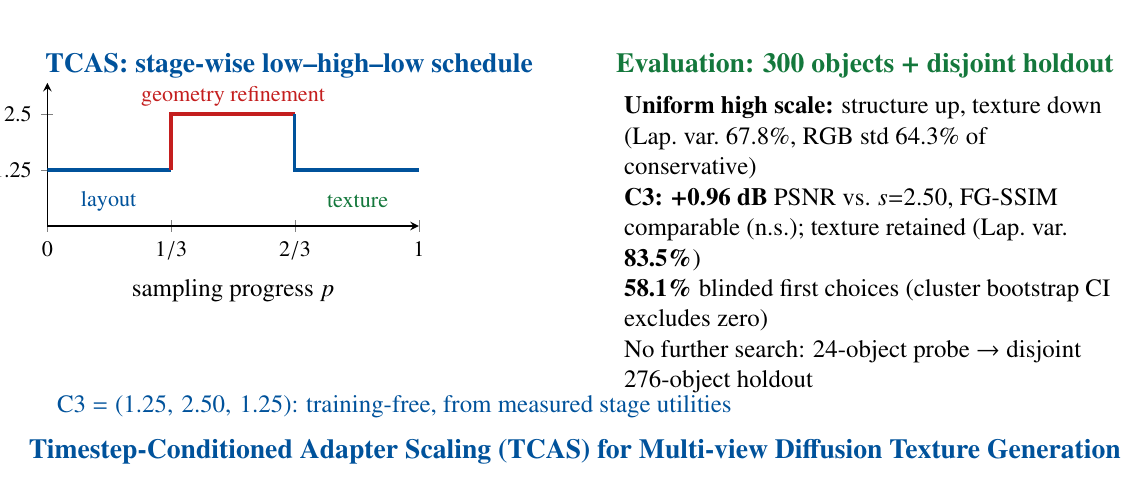
\begin{tikzpicture}[x=1cm,y=1cm,font=\normalsize]
% Fixed-ratio canvas (h:w ~ 0.4 per CAG graphical abstract guideline 531x1328 px)
\useasboundingbox (-0.1,0.2) rectangle (13.75,-5.30);

% ---------------- Left: method core (TCAS schedule) ----------------
\node[anchor=north west, font=\normalsize\bfseries, text=cagblue] at (0,0)
  {TCAS: stage-wise low--high--low schedule};
\begin{scope}[shift={(0.15,-0.5)}]
\begin{axis}[anchor=north west, width=6.3cm, height=3.4cm,
  xlabel={sampling progress $p$}, ylabel={adapter scale $s(p)$},
  xmin=0, xmax=1, ymin=0, ymax=3.2,
  xtick={0,1/3,2/3,1}, xticklabels={$0$,$1/3$,$2/3$,$1$},
  ytick={1.25,2.5}, label style={font=\small}, tick label style={font=\footnotesize},
  axis lines=left]
\addplot[cagblue, very thick] coordinates {(0,1.25)(0.333,1.25)};
\addplot[cagred, very thick] coordinates {(0.333,1.25)(0.333,2.5)(0.666,2.5)};
\addplot[cagblue, very thick] coordinates {(0.666,2.5)(0.666,1.25)(1,1.25)};
\node[font=\footnotesize, text=cagred] at (axis cs:0.5,2.9) {geometry refinement};
\node[font=\footnotesize, text=cagblue] at (axis cs:0.165,0.55) {layout};
\node[font=\footnotesize, text=caggreen] at (axis cs:0.835,0.55) {texture};
\end{axis}
\end{scope}
\node[anchor=north west, font=\small, text=cagblue, align=left] at (0.15,-4.35)
  {C3 $=(1.25,\,2.50,\,1.25)$: training-free, from measured stage utilities};

% ---------------- Right: key results ----------------
\node[anchor=north west, font=\normalsize\bfseries, text=caggreen] at (7.25,0)
  {Evaluation: 300 objects + disjoint holdout};
\node[anchor=north west, align=left, font=\small, text=black] at (7.35,-0.5)
{\begin{tabular}{@{}>{\raggedright\arraybackslash}p{6.2cm}@{}}
\textbf{Uniform high scale:} structure up, texture down (Lap.\ var.\ 67.8\%, RGB std 64.3\% of conservative)\\[3pt]
\textbf{C3:} \textbf{+0.96~dB} PSNR vs.\ $s{=}2.50$, FG-SSIM comparable (n.s.); texture retained (Lap.\ var.\ \textbf{83.5\%})\\[3pt]
\textbf{58.1\%} blinded first choices (cluster bootstrap CI excludes zero)\\[3pt]
No further search: 24-object probe $\to$ disjoint 276-object holdout\\
\end{tabular}};

% ---------------- bottom title ----------------
\node[anchor=north, font=\normalsize\bfseries, text=cagblue] at (6.85,-4.9)
  {Timestep-Conditioned Adapter Scaling (TCAS) for Multi-view Diffusion Texture Generation};

\end{tikzpicture}
\end{document}
